% =============================================================================
%  SIMULACIÓN DE SISTEMAS - TP FINAL
%  Grupo 05 - Sebastián Caules, Andrés Cortese, Tomás J. Esquivel
%  Ampliación a 3D de un simulador peatonal: multiplanta y escaleras.
%  Escenario: Escuela (2 plantas). Estudios: Evacuación e Ingreso.
%
%  Este archivo es el CUERPO compartido por las DOS versiones que pide la cátedra
%  ("la presentación oral debe correr la animación; el PDF entregable lleva
%  fotograma + link a YouTube"):
%
%    * ENTREGABLE  -> compilar ESTE archivo directo:
%        pdflatex SdS_TPFinal_2026Q1G05_Presentacion.tex
%      Sin video embebido: fotograma clickeable + link a YouTube debajo. Liviano.
%
%    * PRESENTABLE -> compilar tpfinal_presentable.tex (define \PRESENTABLEMODE e
%      incluye este cuerpo):
%        pdflatex tpfinal_presentable.tex
%      Video .mp4 EMBEBIDO (reproduce inline en Adobe Acrobat/Reader), SIN links.
%
%  Una sola fuente de contenido -> las dos versiones nunca se desincronizan.
%  Links de YouTube en los macros \videolink... (si se vacían, la versión
%  entregable muestra "[link pendiente]").
%
%  Los videos/posters salen de corridas reales de los barridos (seed 1):
%    videos/anim_evac_n40.mp4     out/sweeps/evacuacion/v40/seed1
%    videos/anim_evac_n120.mp4    out/sweeps/evacuacion/v120/seed1
%    videos/anim_ingreso_t1.mp4   out/sweeps/ingreso/v1/seed1
%    videos/anim_ingreso_t10.mp4  out/sweeps/ingreso/v10/seed1
% =============================================================================

\documentclass[10pt,aspectratio=169,t]{beamer}
\usetheme{Warsaw}
\usecolortheme{default}
\setbeamertemplate{navigation symbols}{}
\useoutertheme{miniframes}

% Footer: solo número de diapositiva a la derecha (igual a TP2/TP3/TP4/TP5)
\setbeamertemplate{footline}{%
    \hfill{\footnotesize\insertframenumber\,/\,\inserttotalframenumber}\hspace{8pt}\vspace{4pt}%
}
\setbeamercolor{frametitle}{bg=blue!70!black, fg=white}

\usepackage[utf8]{inputenc}
\usepackage[T1]{fontenc}
\usepackage[spanish,es-noshorthands]{babel}
\usepackage{amsmath,amssymb,amsfonts}
\usepackage{bm}
\usepackage{graphicx}
\usepackage{booktabs}
\usepackage{siunitx}
\usepackage{xcolor}
\usepackage{tikz}
\usetikzlibrary{arrows.meta,positioning,shapes.geometric,calc}
\usepackage{hyperref}
\usepackage{media9}   % video embebido en el PDF (reproduce inline en Adobe Acrobat/Reader)
\usepackage[absolute,overlay]{textpos}  % anclaje absoluto de la cita (ver \fuente)
\graphicspath{{figuras/}}
\sisetup{output-decimal-marker={.}}

% --- Cita inline en una esquina de la diapositiva (los lineamientos piden las
%     referencias inline, no en una diapositiva final).
%     OJO: NO usar tikz [remember picture, overlay] con current page: el outer
%     theme miniframes rompe ese anclaje. textpos ancla a la página y queda fijo
%     abajo-izquierda también en frames [c] centrados. ---
\newcommand{\fuente}[1]{%
  \begin{textblock*}{0.9\paperwidth}[0,1](0.5cm,\dimexpr\paperheight-0.35cm\relax)
    {\tiny\color{gray} #1}%
  \end{textblock*}}

% --- Links de YouTube/Vimeo a las animaciones. Editar cuando estén subidos. ---
%     Si quedan vacíos, la slide muestra "[link pendiente]" en lugar del URL.
\newcommand{\videolinkEvacBaja}{}     % evacuación, capacidad baja  (N = 40)
\newcommand{\videolinkEvacAlta}{}     % evacuación, capacidad alta  (N = 120)
\newcommand{\videolinkIngresoUno}{}   % ingreso, ventana de 1 minuto
\newcommand{\videolinkIngresoDiez}{}  % ingreso, ventana de 10 minutos

% --- Modo de compilación (lo fija el driver tpfinal_presentable.tex vía
%     \PRESENTABLEMODE; por defecto, compilando este archivo solo, es ENTREGABLE):
%       ENTREGABLE  : \embedvideofalse + \showlinktrue  -> fotograma clickeable
%                     (abre el link) + URL de YouTube visible debajo. Liviano.
%       PRESENTABLE : \embedvideotrue  + \showlinkfalse -> .mp4 embebido (media9,
%                     reproduce inline en Acrobat), SIN URL en pantalla. ---
\newif\ifembedvideo
\newif\ifshowlink
\ifdefined\PRESENTABLEMODE
  \embedvideotrue\showlinkfalse
\else
  \embedvideofalse\showlinktrue
\fi

% --- \simvideo: fotograma/video de una animación.
%     #1 = nombre base en videos/ (espera #1.png y, si embebe, #1.mp4)
%     #2 = link de YouTube (un macro; si está vacío -> "[link pendiente]")
%     Los posters de la vista 3D son ~cuadrados (1056x1044, ancho = 1,0115 alto)
%     -> el tamaño se fija por ALTO (\vidH) y el ancho sale del aspecto. ---
\newlength{\vidH}
\setlength{\vidH}{0.56\textheight}
\makeatletter
\newcommand{\simvideo}[2]{%
  \begin{minipage}{\linewidth}\centering
    \edef\sv@link{#2}% expandimos el link (puede ser un macro vacío)
    \ifembedvideo
      \includemedia[
        activate=onclick,
        width=1.0115\vidH,height=\vidH,
        addresource=videos/#1.mp4,
        flashvars={source=videos/#1.mp4}
      ]{\includegraphics[width=1.0115\vidH,height=\vidH]{videos/#1.png}}{videos/#1.mp4}%
    \else
      \ifx\sv@link\@empty
        \includegraphics[height=\vidH,keepaspectratio]{videos/#1.png}%
      \else
        \href{#2}{\includegraphics[height=\vidH,keepaspectratio]{videos/#1.png}}%
      \fi
    \fi
    \ifshowlink
      \\[2pt]
      {\scriptsize\ttfamily
        \ifx\sv@link\@empty \textcolor{red!60!black}{[link pendiente]}%
        \else \url{#2}\fi}%
    \fi
  \end{minipage}%
}
\makeatother

% --- Metadatos ---
\title[TP Final -- Simulador peatonal 3D]{Ampliación a 3D de un simulador peatonal:\\
  multiplanta y escaleras}
\subtitle{Trabajo Práctico Final}
\author[Caules, Cortese, Esquivel]{Sebastián Caules \and Andrés Cortese \and Tomás J. Esquivel}
\institute[ITBA]{Instituto Tecnológico de Buenos Aires \\ 72.25 -- Simulación de Sistemas -- Grupo 05}
\date{10 de julio de 2026}

\begin{document}

% =============================================================================
% PORTADA
% =============================================================================
{
  \setbeamertemplate{headline}{}
  \setbeamertemplate{footline}{}
  \begin{frame}[plain]
    \titlepage
  \end{frame}
}

% =============================================================================
\section{Ampliación 3D}

\begin{frame}[plain,c]
  \centering
  {\usebeamercolor[fg]{structure}\fontsize{40}{48}\selectfont La ampliación a 3D\\[2pt]
   \large plantas conectadas por escaleras\par}
\end{frame}

\begin{frame}[c]{El objetivo: mapas con más de una planta}
  \begin{columns}[T]
    \begin{column}{0.62\textwidth}
      \begin{itemize}
        \item Punto de partida: un simulador peatonal \textbf{2D} (posición y velocidad
          $(x,y)$ usadas en cascada por todos los módulos).
        \item Objetivo: soportar \textbf{plantas} conectadas por \textbf{escaleras}, y que
          la vecindad, la física, el grafo de navegación y la salida respeten la
          coordenada $z$.
        \item La $z$ representa la \textbf{planta} del agente, y su altura intermedia
          mientras recorre una escalera.
        \item Enfoque \textbf{híbrido}: posiciones y velocidades pasan a 3D, pero la
          dinámica sigue siendo \textbf{planar} en cada planta (evita reescribir la física
          planar y que la $z$ se mueva por fuerzas del plano); la $z$ se interpola por
          el avance sobre la escalera (no hay $v_z$).
      \end{itemize}
    \end{column}
    \begin{column}{0.36\textwidth}
      \centering
      \resizebox{\linewidth}{!}{% Axonometric 3D diagram: two floor slabs connected by a lateral staircase
% (fire-escape style flight glued to the slabs' right face).
% Shared projection contract (do not change x/y/z unit vectors).
% Step recipe twinned with diag_switchback.tex (tramo A): solid body with
% visible risers (-y faces), treads, clean side silhouette with straight
% soffit parallel to the nosing line.
\begin{tikzpicture}[
    scale=0.70,
    x={(0.90cm,-0.30cm)}, y={(0.90cm,0.30cm)}, z={(0cm,0.95cm)},
    line join=round, line cap=round,
    slabtop/.style={fill=blue!8, draw=blue!60!black, thick},
    slabside/.style={fill=blue!20, draw=blue!60!black, thick},
    treadC/.style={fill=orange!40, draw=orange!75!black, thick},
    riserC/.style={fill=orange!60, draw=orange!75!black, thick},
    sideC/.style ={fill=orange!52, draw=orange!75!black, thick},
    aux/.style={gray, densely dashed, thin},
    axisline/.style={gray!70!black, -{Stealth[length=2mm]}, thin},
  ]

  % ---------- geometry constants ----------
  \def\SX{4}\def\SY{3}\def\th{0.25}   % slabs: 4x3 footprint, 0.25 thick
  % staircase: single straight flight attached to the slabs' right face
  % (plane x=\SX), footprint x in [4,5], ascending toward +y so the risers
  % face the viewer (-y) and the stepped silhouette lies on the visible x=5
  % face. 10 steps: rise 0.30 (z 0 -> 3), run 0.24 (y \yA -> \yA+2.4).
  \def\sxo{4.0}\def\sxi{5.0}          % stair width (x range)
  \def\yA{0.20}                       % foot: first riser (front)
  \def\dz{0.30}\def\dy{0.24}          % rise / run per step
  \def\TfV{0.30}                      % vertical height of the top-end cut
  \def\yG{0.44}                       % soffit (slope 1.25) meets ground here

  % ---------- BOTTOM SLAB (floor surface z=0, body z in [-th,0]) ----------
  \draw[slabside] (0,0,-\th) -- (\SX,0,-\th) -- (\SX,0,0) -- (0,0,0) -- cycle;         % -y face
  \draw[slabside] (\SX,0,-\th) -- (\SX,\SY,-\th) -- (\SX,\SY,0) -- (\SX,0,0) -- cycle; % +x face
  \draw[slabtop] (0,0,0) -- (\SX,0,0) -- (\SX,\SY,0) -- (0,\SY,0) -- cycle;            % top

  % ---------- TOP SLAB (floor surface z=3, body z in [3-th,3]) ----------
  \draw[slabside] (0,0,{3-\th}) -- (\SX,0,{3-\th}) -- (\SX,0,3) -- (0,0,3) -- cycle;
  \draw[slabside] (\SX,0,{3-\th}) -- (\SX,\SY,{3-\th}) -- (\SX,\SY,3) -- (\SX,0,3) -- cycle;
  \draw[slabtop] (0,0,3) -- (\SX,0,3) -- (\SX,\SY,3) -- (0,\SY,3) -- cycle;

  % ---------- STAIRCASE (drawn after the slabs: it lies at x > \SX,
  %            i.e. on the viewer side, so it correctly occludes the lower
  %            strips of the slabs' right faces) ----------
  % side silhouette on the visible x=\sxi face: stepped top profile +
  % vertical top-end cut + straight soffit back down to the ground
  \fill[sideC]
    (\sxi,\yA,0)
    foreach \i in {0,...,9} {
      -- (\sxi,{\yA+\i*\dy},{(\i+1)*\dz})
      -- (\sxi,{\yA+(\i+1)*\dy},{(\i+1)*\dz})
    }
    -- (\sxi,{\yA+10*\dy},{3-\TfV})   % top-end cut, under the arrival tread
    -- (\sxi,\yG,0) -- cycle;         % soffit parallel to the nosing line
  % steps, far (top) -> near (foot): riser (visible -y face) + tread
  \foreach \i in {9,8,...,0}{
    \pgfmathsetmacro{\yf}{\yA+\i*\dy}
    \pgfmathsetmacro{\yb}{\yA+(\i+1)*\dy}
    \pgfmathsetmacro{\zl}{\i*\dz}
    \pgfmathsetmacro{\zh}{(\i+1)*\dz}
    \fill[riserC] (\sxo,\yf,\zl) -- (\sxi,\yf,\zl)
          -- (\sxi,\yf,\zh) -- (\sxo,\yf,\zh) -- cycle;   % contrahuella
    \fill[treadC] (\sxo,\yf,\zh) -- (\sxi,\yf,\zh)
          -- (\sxi,\yb,\zh) -- (\sxo,\yb,\zh) -- cycle;   % huella
  }

  % ---------- z axis (subtle height indicator, front-left) ----------
  \draw[axisline] (0,-0.85,-\th) -- (0,-0.85,3.35) node[above,black,font=\scriptsize] {$z$};

  % ---------- AGENTS ----------
  % bottom floor (red)
  \foreach \p in {(1.0,1.0,0),(2.5,1.0,0),(1.6,2.3,0)} {
    \path \p coordinate (a); \fill[red!70!black,draw=white,line width=0.3pt] (a) circle[radius=2.3pt];
  }
  % top floor (green)
  \foreach \p in {(1.1,1.4,3),(2.4,2.1,3)} {
    \path \p coordinate (a); \fill[green!55!black,draw=white,line width=0.3pt] (a) circle[radius=2.3pt];
  }
  % agent in transit on the 5th tread (z=1.5), red like the ground-floor
  % agents (it climbed up from there), slightly larger; dashed vertical
  % down to the z=0 level illustrates its intermediate z
  \path (4.5,1.26,1.56) coordinate (mid);
  \path (4.5,1.26,0) coordinate (midfoot);
  \draw[aux] (mid) -- (midfoot);
  \fill[red!70!black,draw=white,line width=0.3pt] (mid) circle[radius=2.9pt];
  \node[font=\scriptsize,anchor=east,xshift=-8pt,yshift=10pt] at (mid) {$0<z<3$};

  % ---------- LABELS ----------
  \node[font=\scriptsize,anchor=east] at (0,\SY,0) {$z = 0$};
  \node[font=\scriptsize,anchor=east] at (0,\SY,3) {$z = \SI{3}{m}$};
  % "escalera" with a thin leader to the side silhouette (soffit edge);
  % leader routed below the lower slab's silhouette so it crosses nothing
  \draw[gray,thin] (\sxi,0.70,0.325) -- (5.30,0.48,-0.18);
  \node[font=\scriptsize,anchor=north] at (5.30,0.48,-0.18) {escalera};

\end{tikzpicture}
}
    \end{column}
  \end{columns}
\end{frame}

\begin{frame}[c]{Modelo físico: partículas contráctiles (CPM)}
  \begin{itemize}
    \item Cada agente es una partícula de \textbf{radio variable}: se contrae al radio
      mínimo ante un contacto y se re-expande mientras avanza libre.
    \item La velocidad deseada apunta al objetivo, con maniobras angulares de
      \textbf{evitación anisotrópica} (variante A-CPM).
    \item La dinámica ocurre en el \textbf{plano de la planta} del agente; contra las
      paredes sólo interactúa con las de su propia planta.
    \item Sobre la \textbf{escalera}: velocidad reducida por un factor configurable, y la
      $z$ se interpola con el avance a lo largo del tramo.
  \end{itemize}
  \fuente{Refs.: Baglietto \& Parisi, Phys.\ Rev.\ E \textbf{83}, 056117 (2011) ·
    Martin \& Parisi (2024), A-CPM}
\end{frame}

\begin{frame}[c]{Qué cambió en cada módulo, y por qué}
  \footnotesize
  \begin{center}
  \begin{tabular}{@{}p{2.4cm}p{6.2cm}p{4.0cm}@{}}
    \toprule
    \textbf{Módulo} & \textbf{Qué cambió en 3D} & \textbf{Por qué} \\
    \midrule
    Tipos base & Posición y velocidad 3D; la $z$ no es grado de libertad dinámico.
      & La física del CPM es planar. \\
    Geometría & Cada pared, salida, aula y generador lleva su planta; nuevo tipo
      \emph{escalera}. & Un muro pertenece a una planta. \\
    Grafo de navegación & Una malla por planta, unida por \textbf{aristas de escalera};
      A* con heurística euclídea 3D; visibilidad por planta.
      & Una losa tapa la línea de vista entre plantas. \\
    Vecinos (CIM) & Una grilla por planta + índice ``puente'' en la escalera; paredes y
      vértices como vecinos. & El enunciado pide vecindad por planta. \\
    Física (CPM) & Planar en la planta actual; en la escalera, velocidad reducida e
      interpolación de $z$. & La dinámica peatonal ocurre en el plano. \\
    Salida y animación & Columna $z$ en la salida; animación 2D por planta + vista 3D a
      45\textdegree{} apilada. & Ubicar al agente en su planta. \\
    \bottomrule
  \end{tabular}
  \end{center}
\end{frame}

\begin{frame}[c]{Escaleras \emph{switchback} con descanso}
  \begin{columns}[T]
    \begin{column}{0.52\textwidth}
      \begin{itemize}
        \item Tramo en \textbf{L}: dos tramos paralelos unidos por un \textbf{descanso} a
          media altura; se modela como dos escaleras encadenadas $\Rightarrow$ reutiliza
          grafo, vecinos y física sin reescribir el núcleo.
        \item \textbf{Barandas} y el perímetro del descanso confinan al agente dentro de
          la huella.
        \item En tramos anchos, un \emph{bias} lateral separa \textbf{carriles} de subida
          y bajada (contraflujo).
        \item En la vista 3D la escalera se dibuja como un perfil de \textbf{peldaños}.
      \end{itemize}
    \end{column}
    \begin{column}{0.46\textwidth}
      \centering
      \resizebox{\linewidth}{!}{% Escalera switchback con descanso -- vista axonometrica 3D
% Contrato visual compartido: x={(0.90cm,-0.30cm)}, y={(0.90cm,0.30cm)}, z={(0cm,0.95cm)}
% Libs: arrows.meta, calc, 3d
\begin{tikzpicture}[
    x={(0.90cm,-0.30cm)}, y={(0.90cm,0.30cm)}, z={(0cm,0.95cm)},
    line join=round, line cap=round, scale=0.90,
    treadC/.style={fill=orange!40},
    riserC/.style={fill=orange!60},
    sideC/.style ={fill=orange!52},
    edgeO/.style ={draw=orange!75!black},
    slabT/.style ={fill=blue!8},
    slabS/.style ={fill=blue!20},
    edgeB/.style ={draw=blue!60!black}]

  % ---- parametros geometricos (unidades de mundo; z esquematica) ----
  \def\dyy{0.40}\def\dzz{0.30}
  \def\xaA{1.10}\def\xbA{2.05}   % tramo A (frente):  z 0    -> 1.8   (rotulo 1.5 m)
  \def\xaB{0.00}\def\xbB{0.95}   % tramo B (fondo) :  z 1.8  -> 3.6   (rotulo 3 m)
  \def\YY{2.40}                  % 6*dy : borde del descanso
  \def\Zm{1.8}\def\Zt{3.6}       % z mundo del descanso / tope
  \def\Dl{0.68}                  % profundidad del descanso
  \def\tl{0.20}                  % espesor de losa
  \def\Tf{0.44}                  % espesor del tramo B (soffit)

  % =========================================================
  % 1. Piso de referencia (z=0) bajo el pie del tramo A
  % =========================================================
  \fill[blue!6,draw=blue!35,thin]
    (0.95,-0.78,0) -- (2.28,-0.78,0) -- (2.28,0.12,0) -- (0.95,0.12,0) -- cycle;

  % =========================================================
  % 2. Descanso (losa a z=Zm) -- al fondo
  % =========================================================
  \fill[slabS,edgeB,thick] (0.0,\YY,{\Zm-\tl}) -- (\xbA,\YY,{\Zm-\tl})
        -- (\xbA,\YY,\Zm) -- (0.0,\YY,\Zm) -- cycle;                  % cara -y
  \fill[slabS,edgeB,thick] (\xbA,\YY,{\Zm-\tl}) -- (\xbA,{\YY+\Dl},{\Zm-\tl})
        -- (\xbA,{\YY+\Dl},\Zm) -- (\xbA,\YY,\Zm) -- cycle;          % cara +x
  \fill[slabT,edgeB,thick] (0.0,\YY,\Zm) -- (\xbA,\YY,\Zm)
        -- (\xbA,{\YY+\Dl},\Zm) -- (0.0,{\YY+\Dl},\Zm) -- cycle;     % cara superior

  % =========================================================
  % 3. Tramo B (fondo): losa escalonada inclinada z=Zm -> Zt
  %    (riseres miran +y = ocultos; se ve cara +x interna + huellas)
  % =========================================================
  \fill[sideC,edgeO,thick]
    (\xbB,\YY,\Zm)
    foreach \j in {0,...,5} {
       -- (\xbB,{\YY-\j*\dyy},{\Zm+(\j+1)*\dzz})
       -- (\xbB,{\YY-(\j+1)*\dyy},{\Zm+(\j+1)*\dzz})
    }
    -- (\xbB,0,{\Zt-\Tf}) -- (\xbB,\YY,{\Zm-\Tf}) -- cycle;
  % huellas del tramo B (k=1 lejos -> k=6 cerca)
  \foreach \k in {1,...,6}{
    \pgfmathsetmacro{\zt}{\Zm+\k*\dzz}
    \pgfmathsetmacro{\yfr}{\YY-\k*\dyy}
    \pgfmathsetmacro{\ybk}{\YY-(\k-1)*\dyy}
    \fill[treadC,edgeO,thick] (\xaB,\yfr,\zt) -- (\xbB,\yfr,\zt)
          -- (\xbB,\ybk,\zt) -- (\xaB,\ybk,\zt) -- cycle;
  }
  \fill[riserC,edgeO,thick] (\xaB,0,{\Zt-\Tf}) -- (\xbB,0,{\Zt-\Tf})
        -- (\xbB,0,\Zt) -- (\xaB,0,\Zt) -- cycle;                    % tapa -y del tope
  % perfil escalonado en negrita sobre la cara +x visible (para que se lean peldanos)
  \draw[orange!75!black,thick]
    (\xbB,\YY,\Zm)
    foreach \j in {0,...,5} {
       -- (\xbB,{\YY-\j*\dyy},{\Zm+(\j+1)*\dzz})
       -- (\xbB,{\YY-(\j+1)*\dyy},{\Zm+(\j+1)*\dzz})
    };

  % =========================================================
  % 4. Tramo A (frente): escalera solida z=0 -> Zm
  % =========================================================
  \fill[sideC,edgeO,thick]
    (\xbA,0,0)
    foreach \i in {0,...,5} {
       -- (\xbA,{\i*\dyy},{(\i+1)*\dzz})
       -- (\xbA,{(\i+1)*\dyy},{(\i+1)*\dzz})
    }
    -- (\xbA,\YY,0) -- cycle;
  \foreach \i in {5,4,3,2,1,0}{
    \pgfmathsetmacro{\yf}{\i*\dyy}
    \pgfmathsetmacro{\yb}{(\i+1)*\dyy}
    \pgfmathsetmacro{\zl}{\i*\dzz}
    \pgfmathsetmacro{\zh}{(\i+1)*\dzz}
    \fill[riserC,edgeO,thick] (\xaA,\yf,\zl) -- (\xbA,\yf,\zl)
          -- (\xbA,\yf,\zh) -- (\xaA,\yf,\zh) -- cycle;              % contrahuella
    \fill[treadC,edgeO,thick] (\xaA,\yf,\zh) -- (\xbA,\yf,\zh)
          -- (\xbA,\yb,\zh) -- (\xaA,\yb,\zh) -- cycle;              % huella
  }

  % =========================================================
  % 5. Fragmento de losa de la planta alta (z=Zt) en el tope
  % =========================================================
  \def\ua{-0.15}\def\ub{1.05}\def\va{-0.68}\def\vb{0.00}
  \fill[slabS,edgeB,thick] (\ua,\va,{\Zt-\tl}) -- (\ub,\va,{\Zt-\tl})
        -- (\ub,\va,\Zt) -- (\ua,\va,\Zt) -- cycle;                  % cara -y
  \fill[slabS,edgeB,thick] (\ub,\va,{\Zt-\tl}) -- (\ub,\vb,{\Zt-\tl})
        -- (\ub,\vb,\Zt) -- (\ub,\va,\Zt) -- cycle;                  % cara +x
  \fill[slabT,edgeB,thick] (\ua,\va,\Zt) -- (\ub,\va,\Zt)
        -- (\ub,\vb,\Zt) -- (\ua,\vb,\Zt) -- cycle;                  % cara superior

  % =========================================================
  % 6. Barandas: omitidas a proposito. En esta proyeccion, todo
  %    pasamanos paralelo a la pendiente proyecta casi paralelo a la
  %    flecha de recorrido (<2 mm de holgura en pagina) y se enreda
  %    con ella; el confinamiento por barandas ya lo dice el texto
  %    de la slide.
  % =========================================================

  % =========================================================
  % 7. Flecha de recorrido (elemento narrativo) -- muy gruesa
  % =========================================================
  \def\xcA{1.575}\def\xcB{0.475}
  \draw[-{Latex[length=2.8mm,width=2.8mm]},line width=1.7pt,blue!60!black]
     (\xcA,0.12,0.35) -- (\xcA,1.70,1.36);                          % sube tramo A (waypoint)
  \draw[-{Latex[length=2.8mm,width=2.8mm]},line width=1.7pt,blue!60!black]  % remate A + giro 180 + tramo B
     (\xcA,1.86,1.46) -- (\xcA,{\YY+0.06},{\Zm+0.05})
     .. controls (\xcA,{\YY+\Dl+0.12},{\Zm+0.05}) and (\xcB,{\YY+\Dl+0.12},{\Zm+0.05}) ..
     (\xcB,{\YY+0.06},{\Zm+0.05}) -- (\xcB,0.15,{\Zt+0.08});

  % =========================================================
  % 8. Etiquetas con lineas lider (scriptsize)
  % =========================================================
  % pie -- debajo del pie del tramo A
  \draw[gray,thin] (1.58,0.06,0.05) -- (1.30,-0.60,0.05);
  \node[anchor=north,font=\scriptsize] at (1.30,-0.60,0.05) {pie ($z=0$)};
  % descanso -- abajo-derecha, hacia el borde frontal-derecho del descanso
  \draw[gray,thin] (\xbA,{\YY+0.10},\Zm) -- (2.05,{\YY-0.30},0.62);
  \node[anchor=west,font=\scriptsize] at (2.05,{\YY-0.30},0.62) {descanso ($z=\SI{1.5}{m}$)};
  % tope -- arriba del tope del tramo B
  \draw[gray,thin] (0.35,0.05,\Zt) -- (0.62,-0.42,{\Zt+0.32});
  \node[anchor=south,font=\scriptsize] at (0.62,-0.42,{\Zt+0.32}) {tope ($z=\SI{3}{m}$)};

\end{tikzpicture}
}
    \end{column}
  \end{columns}
\end{frame}

\begin{frame}[c]{Lo que sólo aparece con dos plantas reales}
  \begin{itemize}
    \item \textbf{Verde en aislamiento, roto en integración}: cada módulo pasaba sus
      tests, pero el primer escenario real de dos plantas destapó caminos donde la $z$ se
      perdía \emph{en silencio} (tareas, servers y generadores nacían o apuntaban a
      $z=0$): nadie subía a la planta alta, y sin un solo \emph{crash}.
    \item \textbf{El ruteo se quedaba al pie} de la escalera (el tope ``no es visible''
      desde otra planta) $\Rightarrow$ se cruza explícitamente la \textbf{arista de
      escalera}.
    \item \textbf{Salto de $z$ al pie}: se excluyó la huella de la escalera de la grilla
      del grafo y el cambio de \emph{hop} se hace pegado al extremo, para que la $z$
      enganche desde el nivel del piso.
    \item \textbf{Livelock en jambas de puerta}: el contacto con pared al radio expandido
      disparaba un escape que peleaba con el objetivo $\Rightarrow$ contacto sólo al
      núcleo duro ($r_{\min}$); la repulsión suave dobla esquinas sin oscilar.
    \item \textbf{Lección}: al agregar una coordenada hay que auditar \emph{todos} los
      caminos de datos; los \emph{defaults} silenciosos dan simulaciones plausibles pero
      erróneas.
  \end{itemize}
\end{frame}

% =============================================================================
\section{Escuela}

\begin{frame}[plain,c]
  \centering
  {\usebeamercolor[fg]{structure}\fontsize{40}{48}\selectfont Escenario: Escuela\par}
\end{frame}

\begin{frame}[c]{El mapa: recreo y edificio de dos plantas}
  \begin{columns}[T]
    \begin{column}{0.46\textwidth}
      \centering
      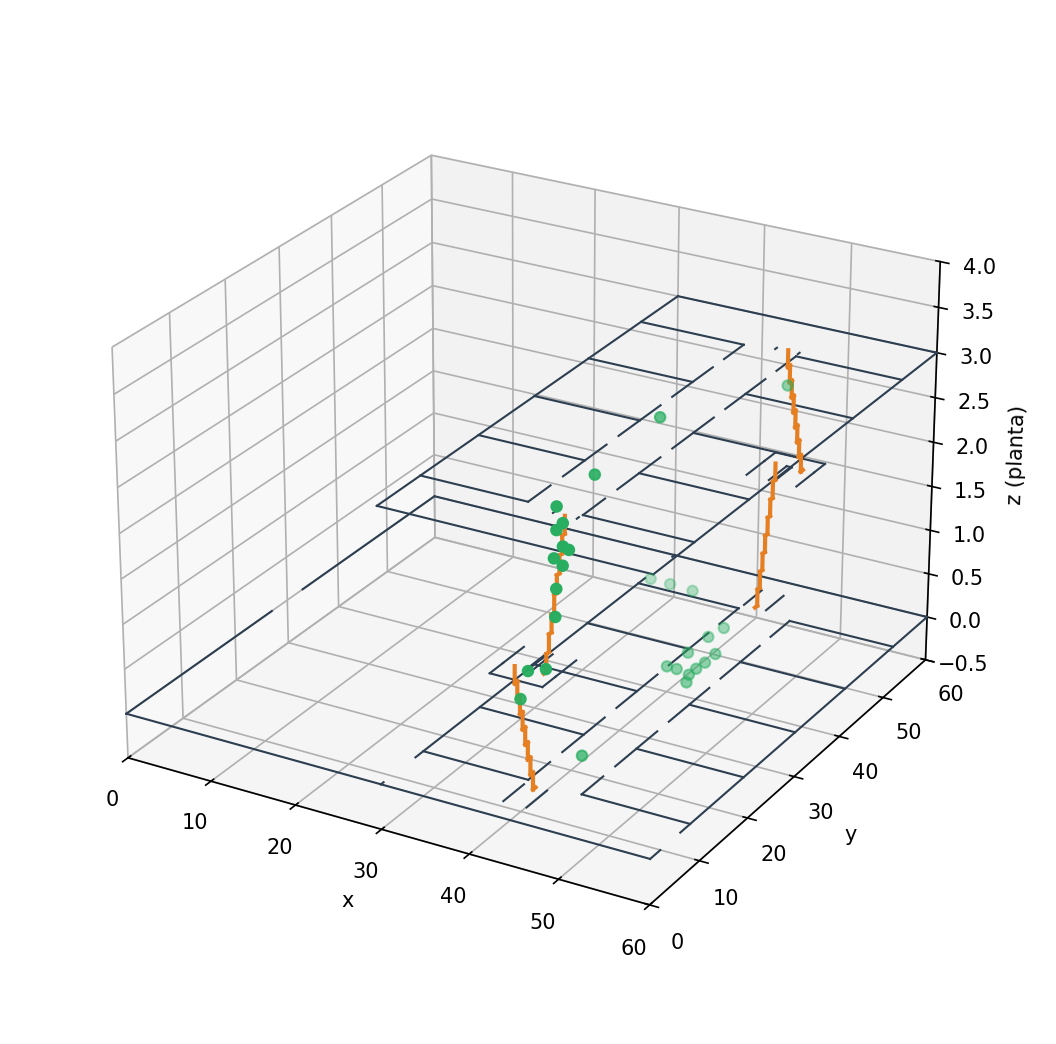
\includegraphics[width=\linewidth,height=0.72\textheight,keepaspectratio]{escuela_3d.png}\\
      {\footnotesize Vista 3D apilada: planta baja, descanso y planta alta.}
    \end{column}
    \begin{column}{0.52\textwidth}
      \begin{itemize}
        \item Mapa de \SI{60}{m}$\times$\SI{60}{m} con dos zonas.
        \item \textbf{Recreo} (una planta): patio abierto, \textbf{kiosco} con cola y
          salida propia.
        \item \textbf{Edificio} (dos plantas): pasillo central, \textbf{16 aulas}
          (4 por lado y por planta) y \textbf{dos escaleras switchback} en las puntas.
        \item La planta alta \textbf{no tiene salida}: se evacúa bajando por las
          escaleras.
        \item Las aulas son recintos colectivos con una sesión de clase y timbre
          único de salida.
      \end{itemize}
    \end{column}
  \end{columns}
\end{frame}

\begin{frame}[c]{Parámetros de las corridas}
  \begin{columns}[T]
    \begin{column}{0.52\textwidth}
      \textbf{Agentes (perfil CPM)}
      \begin{itemize}
        \item Radios: $r_{\min}=\SI{0.15}{m}$, $r_{\max}\sim\mathcal{U}(0.30,0.32)\,$m;
          $\tau=\SI{0.5}{s}$; $\beta=0.9$.
        \item Caminata normal: $v_d=\SI{1.55}{m/s}$.
        \item \textbf{Modo crisis} (evacuación): $v_d=v_e=\SI{2.0}{m/s}$, como en los
          modelos de escape.
      \end{itemize}
    \end{column}
    \begin{column}{0.46\textwidth}
      \textbf{Simulación}
      \begin{itemize}
        \item $\Delta t$ acotado por el perfil más rápido: \SI{0.048}{s}
          (\SI{0.0375}{s} en evacuación); $\Delta t_{\text{out}}=\SI{0.2}{s}$.
        \item Escalera: ancho \SI{2.6}{m}; velocidad efectiva en el tramo
          $\approx\SI{0.59}{m/s}$.
        \item \textbf{5 realizaciones} por punto (semillas 1--5): la semilla global
          gobierna todos los procesos aleatorios (spawn, ruteo, elección de salida/aula,
          tiempos de servicio) $\Rightarrow$ realizaciones independientes. Se reporta
          media $\pm\,\sigma$, con barras de error.
      \end{itemize}
    \end{column}
  \end{columns}
  \fuente{Perfil: Baglietto \& Parisi (2011) · Velocidad de crisis: Helbing, Farkas
    \& Vicsek, Nature \textbf{407} (2000)}
\end{frame}

% =============================================================================
\section{Evacuación}

\begin{frame}[plain,c]
  \centering
  {\usebeamercolor[fg]{structure}\fontsize{40}{48}\selectfont Estudio 1: Evacuación\par}
\end{frame}

\begin{frame}[c]{Qué medimos en la evacuación}
  \begin{itemize}
    \item Los $N$ alumnos comienzan \textbf{dentro de las aulas} de ambas plantas y
      evacúan en \textbf{modo crisis} hacia las dos salidas; los de la planta alta bajan
      por las escaleras.
    \item \textbf{Input}: la capacidad total $N \in \{40, 80, 120\}$.
    \item \textbf{Observable}: la distribución de los tiempos de evacuación
      \begin{equation*}
        t_{\text{evac},i} \;=\; t_{\text{salida},i} - t_{\text{inicio},i}.
      \end{equation*}
    \item \textbf{Escalares}: $t_{\text{evac}}$ \textbf{promedio} y \textbf{máximo} en
      función de $N$.
  \end{itemize}
\end{frame}

\begin{frame}[c]{La evacuación desde ambas plantas}
  \begin{columns}[T]
    \begin{column}{0.5\textwidth}
      \centering
      \simvideo{anim_evac_n40}{\videolinkEvacBaja}\\[1pt]
      {\footnotesize Capacidad baja: $N=40$.}
    \end{column}
    \begin{column}{0.5\textwidth}
      \centering
      \simvideo{anim_evac_n120}{\videolinkEvacAlta}\\[1pt]
      {\footnotesize Capacidad alta: $N=120$.}
    \end{column}
  \end{columns}
\end{frame}

\begin{frame}[c]{La distribución de tiempos de evacuación es bimodal}
  \centering
  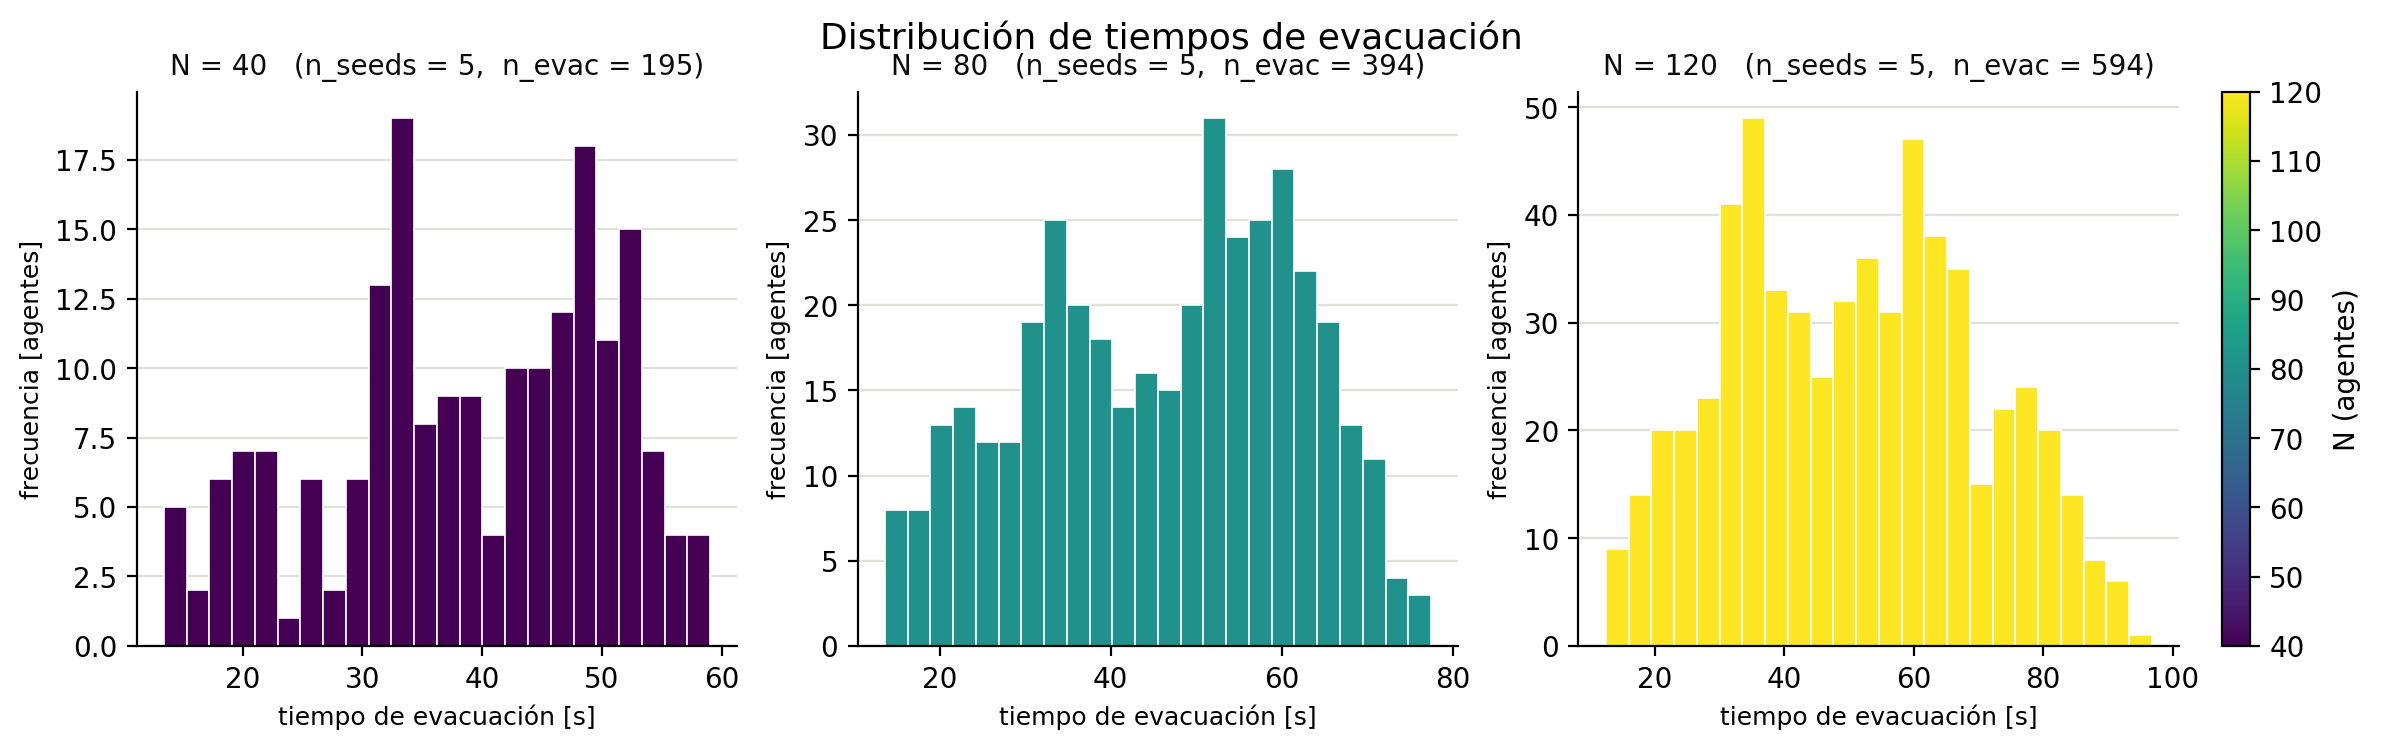
\includegraphics[width=0.95\linewidth]{evac_hist.png}\\[4pt]
  \begin{itemize}
    \item El lóbulo rápido es la \textbf{planta baja}; el lento, la \textbf{planta alta},
      que debe bajar la escalera a velocidad reducida.
    \item Al crecer $N$, el lóbulo lento se desplaza a tiempos mayores y produce la cola
      larga.
  \end{itemize}
\end{frame}

\begin{frame}[c]{El tiempo de evacuación crece con la capacidad}
  \begin{columns}[T]
    \begin{column}{0.56\textwidth}
      \centering
      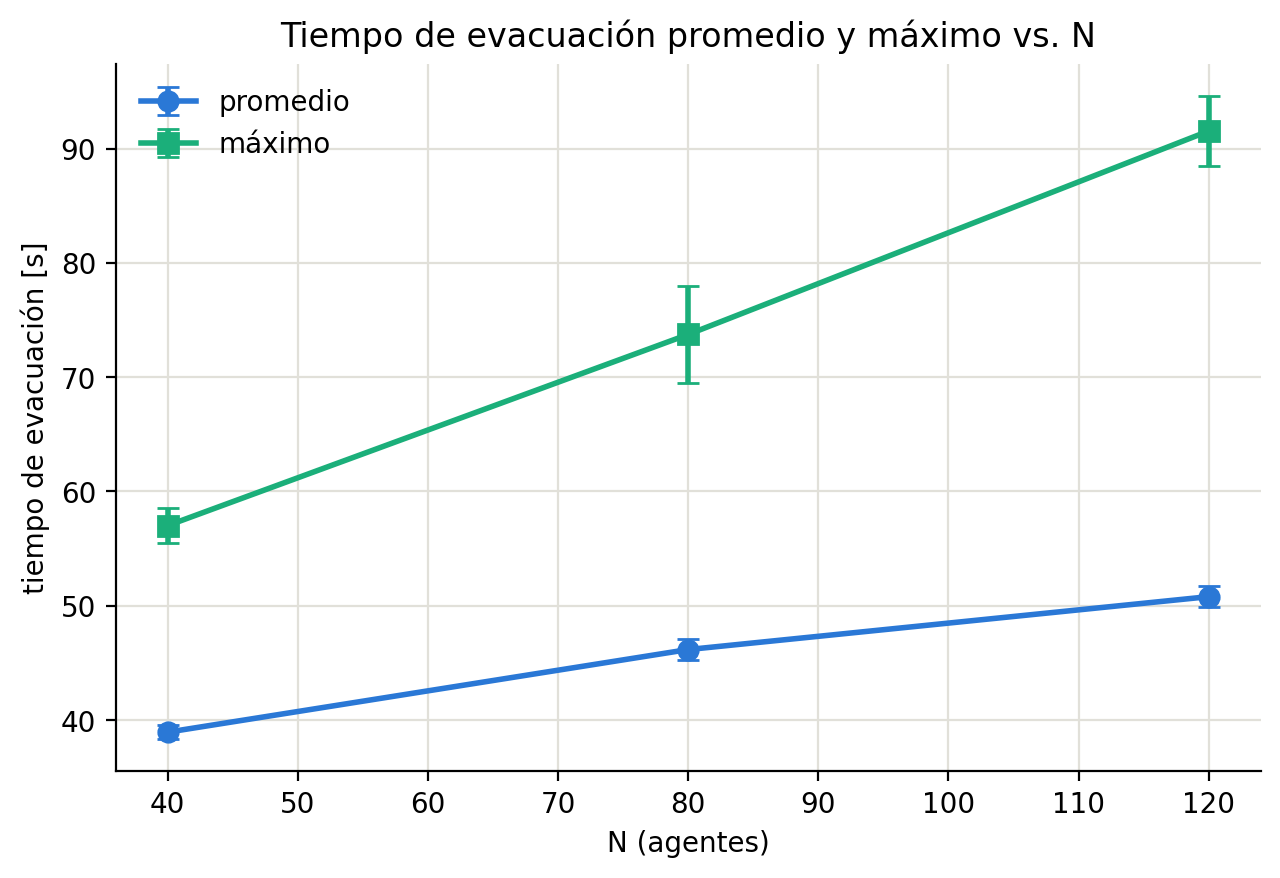
\includegraphics[width=\linewidth,height=0.74\textheight,keepaspectratio]{evac_scalar.png}
    \end{column}
    \begin{column}{0.42\textwidth}
      \textbf{Observaciones}
      \begin{itemize}
        \item Al triplicar la capacidad, el promedio pasa de $38.9\pm0.6$ a
          $50.8\pm0.9$~s y el máximo de $57.0\pm1.5$ a $91.5\pm3.1$~s.
        \item La dispersión entre realizaciones crece con $N$: más congestión, más
          sensibilidad a la realización.
        \item Barras de error: $\pm\,\sigma$ entre las 5 realizaciones (dentro del
          marcador donde no se ven).
        \item Queda $\approx 1$ agente por corrida sin evacuar: casi siempre el último
          en tránsito a la salida (borde del criterio); la escalera fluye sin atascos.
      \end{itemize}
    \end{column}
  \end{columns}
\end{frame}

\begin{frame}[c]{La huella espacial de la evacuación}
  \begin{columns}[T]
    \begin{column}{0.5\textwidth}
      \centering
      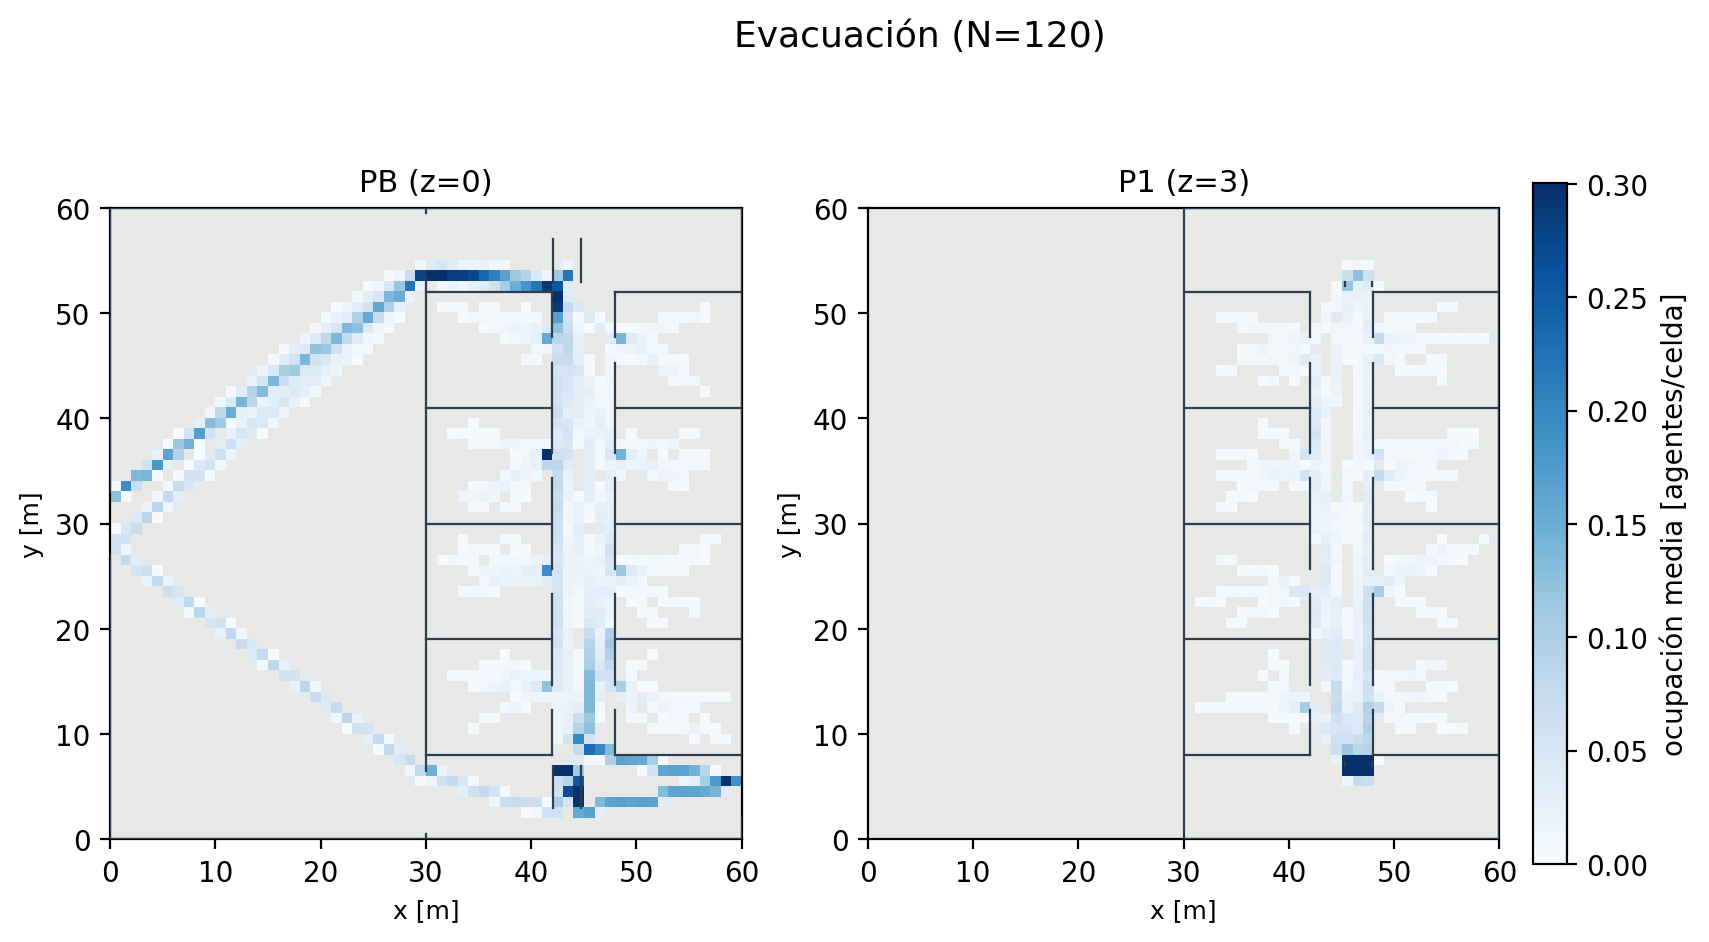
\includegraphics[width=\linewidth]{heatmap_densidad_evac.png}\\[2pt]
      {\footnotesize Densidad de ocupación: el pasillo central y las escaleras
        concentran el flujo.}
    \end{column}
    \begin{column}{0.5\textwidth}
      \centering
      
\includegraphics[width=\linewidth]{heatmap_tevac.png}\\[2pt]
      {\footnotesize $t_{\text{evac}}$ medio según el origen: la planta alta evacúa
        mucho más lento (baja por escalera).}
    \end{column}
  \end{columns}
\end{frame}

% =============================================================================
\section{Ingreso}

\begin{frame}[plain,c]
  \centering
  {\usebeamercolor[fg]{structure}\fontsize{40}{48}\selectfont Estudio 2: Ingreso\par}
\end{frame}

\begin{frame}[c]{Qué medimos en el ingreso}
  \begin{itemize}
    \item Los $N_{\max}=120$ alumnos llegan repartidos uniformemente en una
      \textbf{ventana} $T_a \in \{1, 5, 10\}$~min y van a sus aulas; los que entran por
      el recreo pasan antes por el \textbf{kiosco}.
    \item \textbf{Input}: la ventana $T_a$, equivalente a un caudal
      $Q = N_{\max}/T_a \in \{120, 24, 12\}$ agentes/min.
    \item \textbf{Observable}: la población en la zona del kiosco
      \begin{equation*}
        n_{\text{zona}}(t) \;=\; \bigl|\{\, i : (x_i(t), y_i(t)) \in R \,\}\bigr|,
        \qquad R = \text{frente del kiosco (planta baja)}.
      \end{equation*}
    \item \textbf{Escalares}: ocupación \textbf{máxima} y \textbf{promedio} de la zona.
    \item ¿Por qué el kiosco? El pie de la escalera no congestiona (switchback ancha,
      dos escaleras, sólo la mitad sube): la congestión real se forma \textbf{frente al
      kiosco}.
  \end{itemize}
\end{frame}

\begin{frame}[c]{La congestión se forma frente al kiosco}
  \begin{columns}[T]
    \begin{column}{0.5\textwidth}
      \centering
      \simvideo{anim_ingreso_t1}{\videolinkIngresoUno}\\[1pt]
      {\footnotesize Ventana corta: $T_a=\SI{1}{min}$ ($Q=120$ ag/min).}
    \end{column}
    \begin{column}{0.5\textwidth}
      \centering
      \simvideo{anim_ingreso_t10}{\videolinkIngresoDiez}\\[1pt]
      {\footnotesize Ventana larga: $T_a=\SI{10}{min}$ ($Q=12$ ag/min).}
    \end{column}
  \end{columns}
\end{frame}

\begin{frame}[c]{Población en el kiosco durante el ingreso}
  \begin{columns}[T]
    \begin{column}{0.62\textwidth}
      \centering
      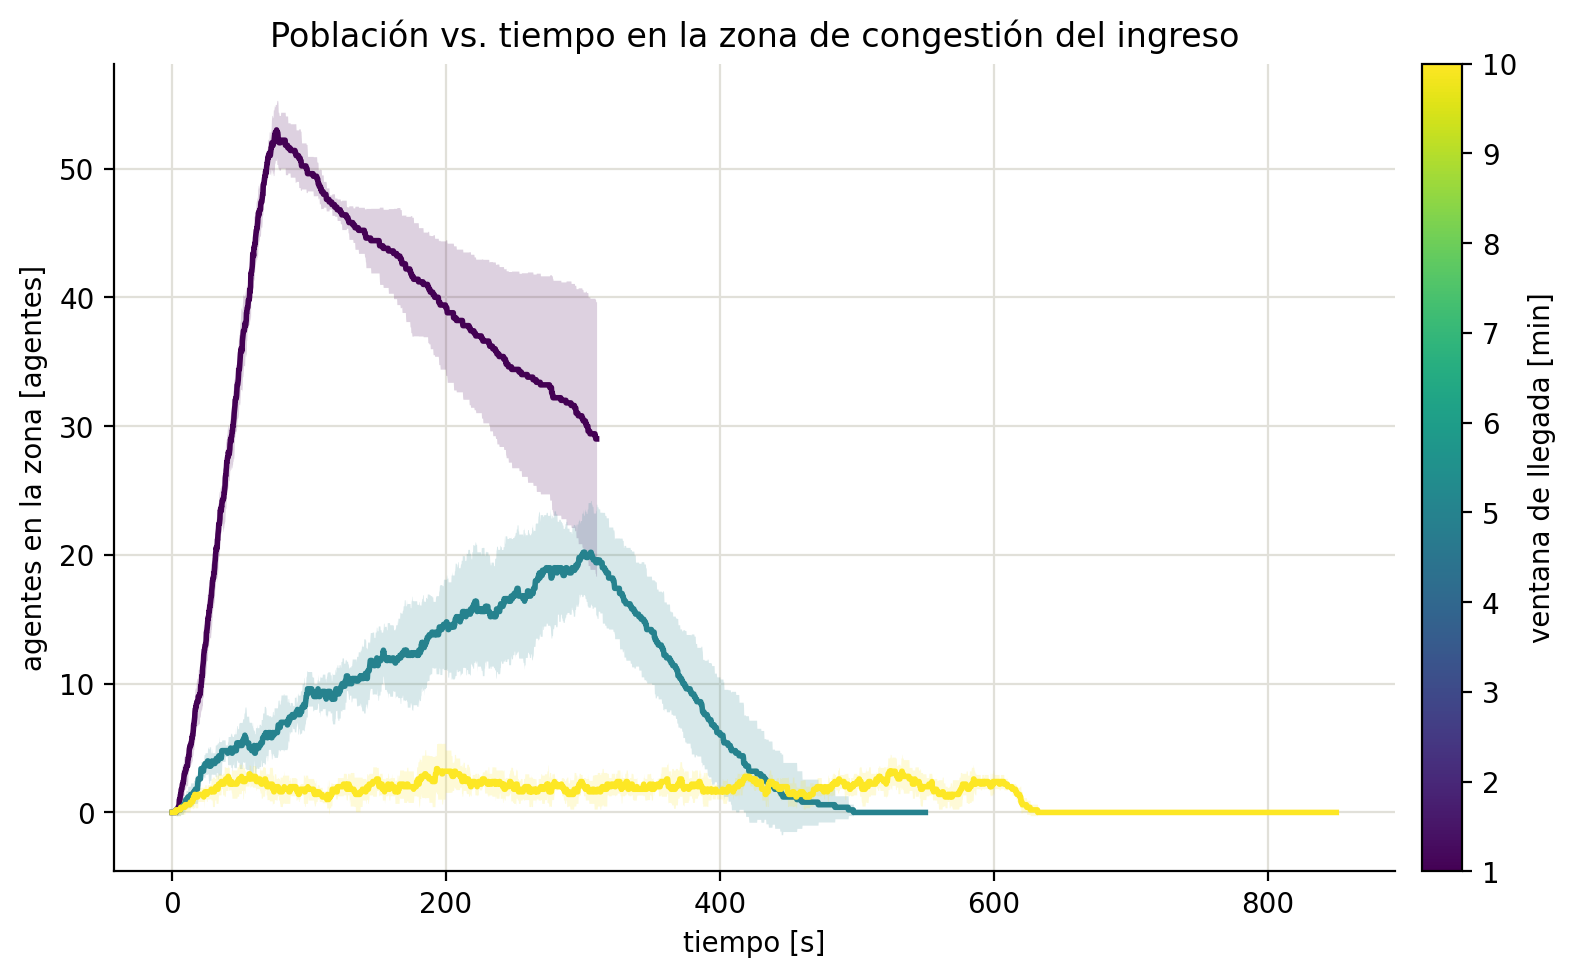
\includegraphics[width=\linewidth,height=0.76\textheight,keepaspectratio]{ingreso_poblacion.png}
    \end{column}
    \begin{column}{0.36\textwidth}
      \textbf{Observaciones}
      \begin{itemize}
        \item Ventana corta: pico \textbf{agudo y temprano}; ventana larga: meseta
          \textbf{baja y extendida}.
        \item El mismo total de personas, distinta intensidad de aglomeración.
        \item La banda sombreada es $\pm\,\sigma$ entre las 5 realizaciones.
      \end{itemize}
    \end{column}
  \end{columns}
\end{frame}

\begin{frame}[c]{Repartir la llegada descongestiona la zona}
  \begin{columns}[T]
    \begin{column}{0.56\textwidth}
      \centering
      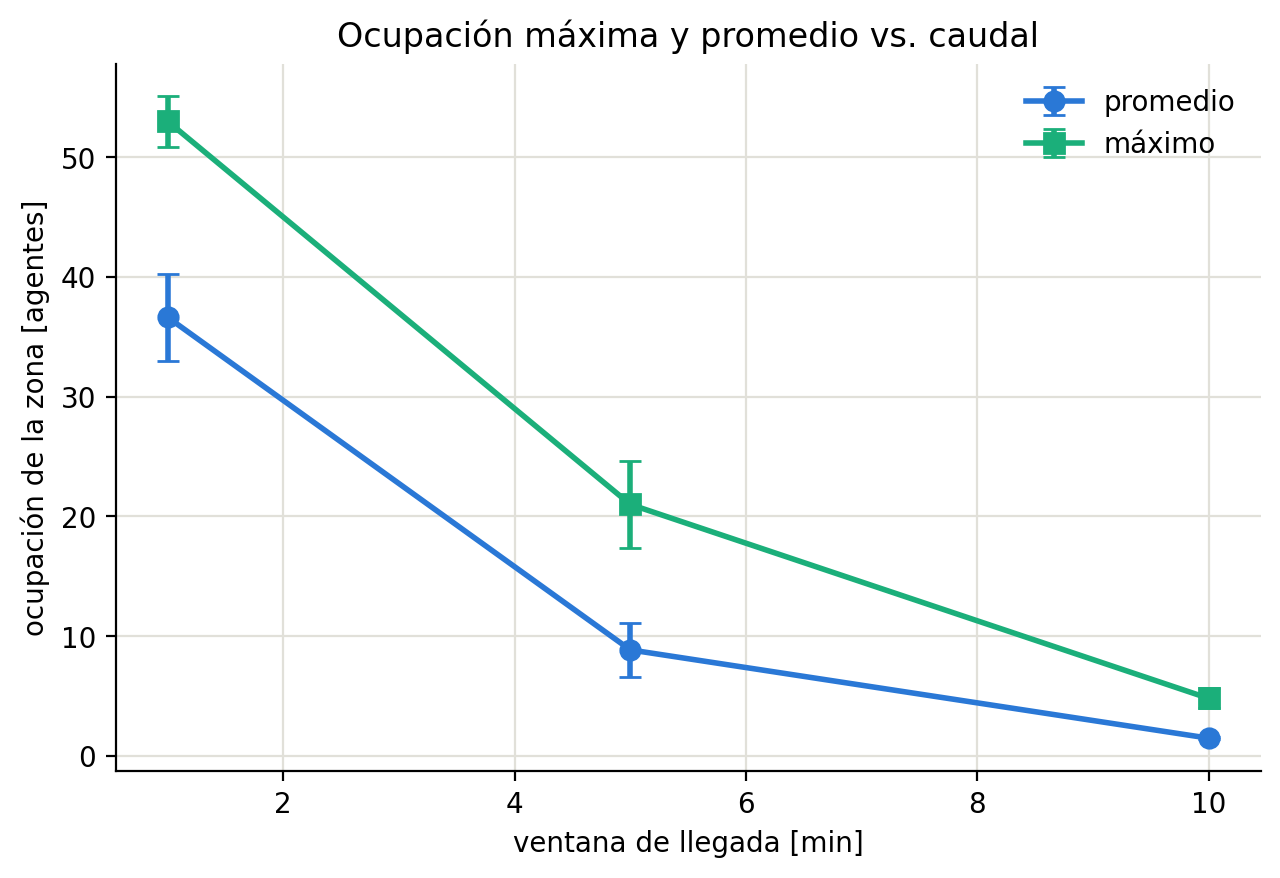
\includegraphics[width=\linewidth,height=0.74\textheight,keepaspectratio]{ingreso_scalar.png}
    \end{column}
    \begin{column}{0.42\textwidth}
      \textbf{Observaciones}
      \begin{itemize}
        \item Concentrar la llegada en \SI{1}{min} produce un pico de $53.0\pm2.1$
          agentes; repartirla en \SI{10}{min} lo baja a $4.8\pm0.8$
          ($\sim$11$\times$ menos).
        \item Con la ventana de \SI{1}{min} la cola del kiosco no llega a drenarse en
          la corrida: el servidor queda \textbf{saturado}.
        \item Donde las barras de error no se distinguen, son menores que el marcador.
      \end{itemize}
    \end{column}
  \end{columns}
\end{frame}

\begin{frame}[c]{Estudio complementario: la congestión crece con la cantidad de alumnos}
  \begin{columns}[T]
    \begin{column}{0.54\textwidth}
      \centering
      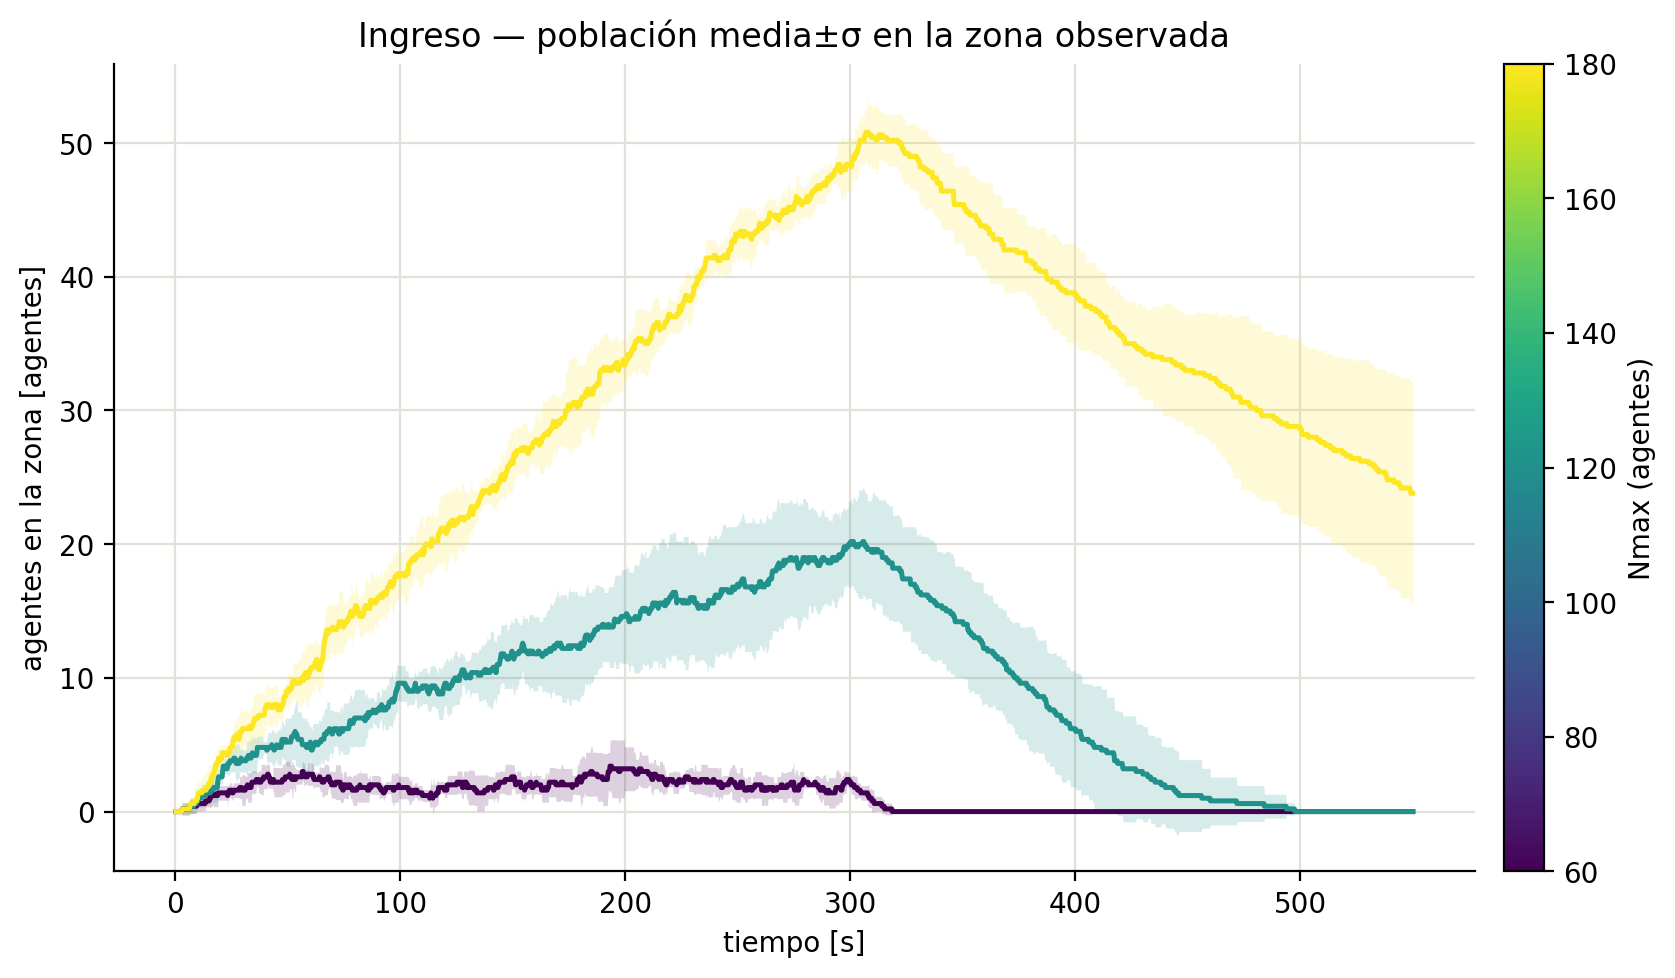
\includegraphics[width=\linewidth,height=0.62\textheight,keepaspectratio]{ingreso_nmax_poblacion.png}
    \end{column}
    \begin{column}{0.44\textwidth}
      \centering
      
\includegraphics[width=\linewidth,height=0.62\textheight,keepaspectratio]{ingreso_nmax_scalar.png}
    \end{column}
  \end{columns}
  \vspace{2pt}
  \begin{itemize}
    \item A ventana fija, se varía la cantidad total $N_{\max}\in\{60,120,180\}$.
    \item Triplicar $N_{\max}$ multiplica el pico $\sim$11$\times$ ($4.6 \to 51.4$): la
      ocupación crece \textbf{más que proporcionalmente} en el rango explorado.
  \end{itemize}
\end{frame}

\begin{frame}[c]{La huella espacial del ingreso}
  \centering
  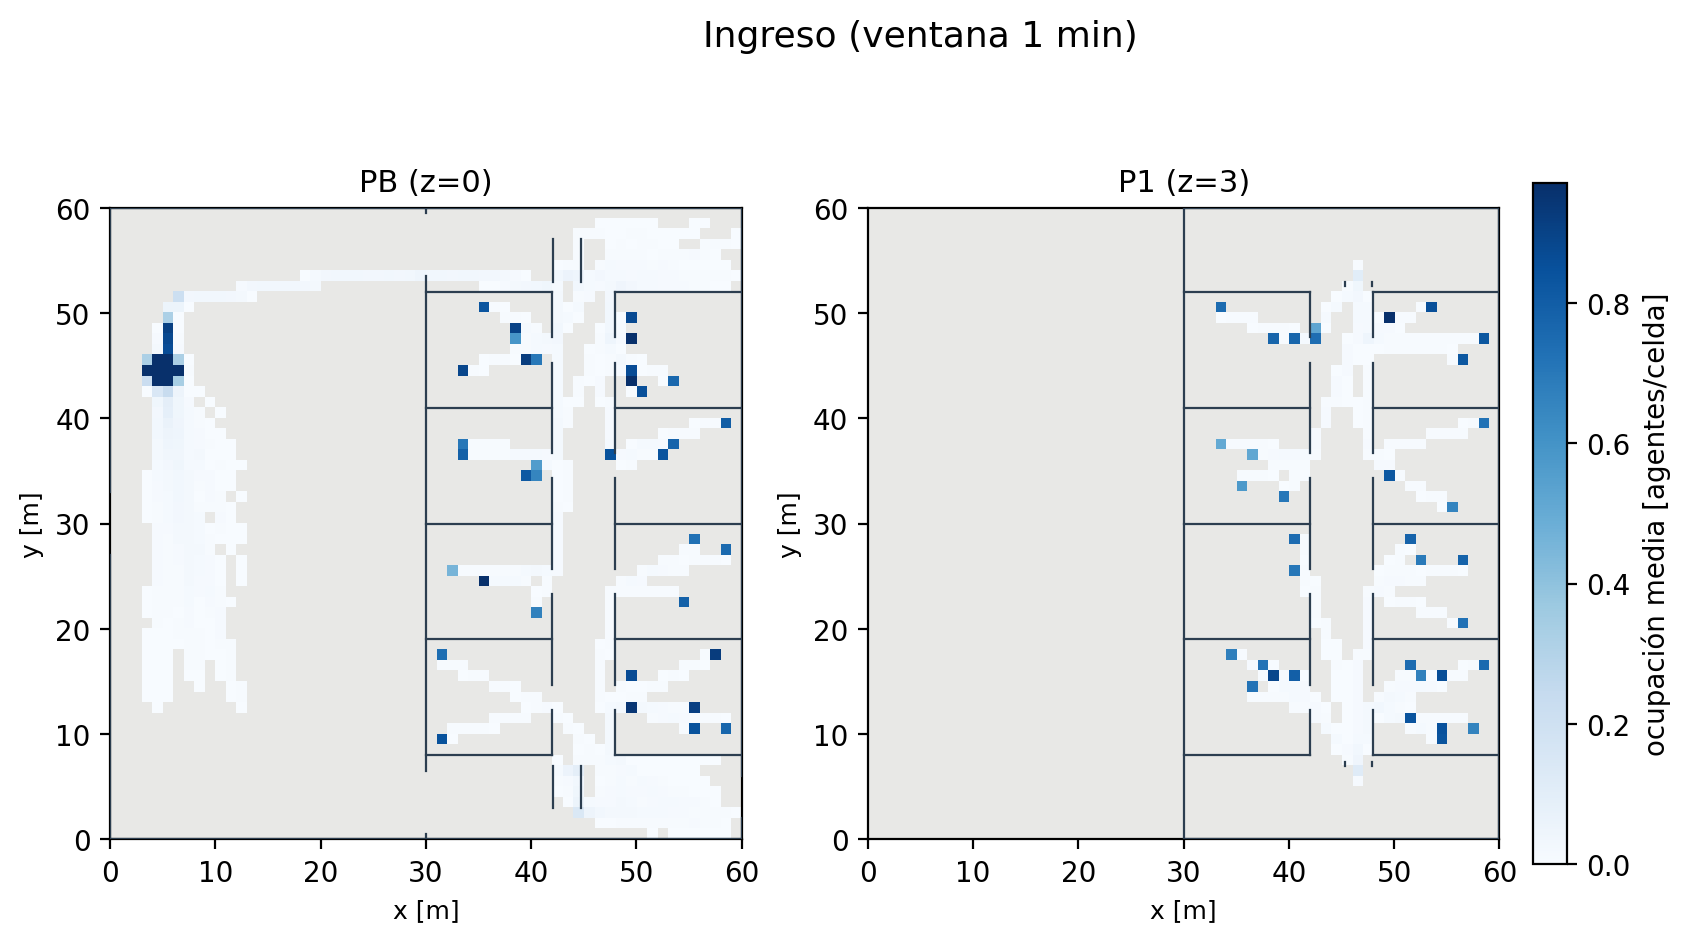
\includegraphics[width=0.8\linewidth,height=0.68\textheight,keepaspectratio]{heatmap_densidad_ingreso.png}\\[3pt]
  {\footnotesize Densidad de ocupación durante el ingreso: la cola del kiosco es el punto
    caliente; pasillos y entradas quedan mucho más tenues.}
\end{frame}

% =============================================================================
\section{Conclusiones}

\begin{frame}[plain,c]
  \centering
  {\usebeamercolor[fg]{structure}\fontsize{40}{48}\selectfont Conclusiones\par}
\end{frame}

\begin{frame}[c]{Conclusiones}
  \begin{itemize}
    \item El simulador quedó ampliado a 3D \textbf{de punta a punta}: agentes que
      recorren escaleras a velocidad reducida, vecinos y física por planta, grafo de
      navegación 3D, y animación por planta más vista 3D apilada.
    \item La escalera \textbf{switchback} con descanso, confinamiento y carriles de
      contraflujo da un comportamiento coherente.
    \item El \textbf{tiempo de evacuación crece con la capacidad}, y su distribución es
      \textbf{bimodal}: la planta baja sale rápido y la planta alta forma el lóbulo
      lento.
    \item La \textbf{ocupación del kiosco crece al acortar la ventana de llegada} y, a
      ventana fija, crece más que proporcionalmente con la cantidad de alumnos, en el
      rango explorado.
    \item Límite conocido: $\approx 1$ agente por corrida no evacúa (casi siempre el último
      en tránsito; esporádicamente el \emph{livelock} de contacto con muros del CPM en un
      portón de PB). El descenso por la escalera fluye sin atascos.
  \end{itemize}
\end{frame}

% =============================================================================
{
  \setbeamertemplate{footline}{}
  \begin{frame}[plain,c]
    \centering
    {\fontsize{44}{52}\selectfont Muchas gracias\par}
  \end{frame}
}

\end{document}
